\section{Importación, Exploración y Limpieza de los Datos} \label{section:depuracion}

Se realiza la carga de las librerías e importación del conjunto de datos \texttt{sales.csv}, obtenido de \href{https://www.kaggle.com/datasets/sudipmanchare/simulated-sales-data-with-timeseries-features}{Kaggle}. Se utiliza el siguiente código.

\begin{lstlisting}
	train = pd.read_csv("sales.csv")
	print(train.head())
	if (train.isna().sum().sum() > 0):
	print(train.isna().sum())
	train.info()
\end{lstlisting}

El conjunto de datos contiene 365 registros por columna y no presenta valores faltantes. Esto equivale a 365 días de datos.
 Sin embargo, cuenta con tres columnas, mientras que para la creación de una serie temporal solo se requieren dos: una para el tiempo y otra como variable predictora.\\

\begin{figure}[h]
	\centering
	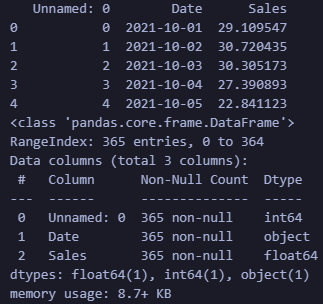
\includegraphics[width=0.3\linewidth]{train_info}
	\caption{Conjunto de Datos Original}
	\label{fig:traininfo}
\end{figure}

El código que se muestra a continuación es el utilizado para eliminar la columna sobrante $Unnamed: 0$ y asignar a la variable $Date$ convertida en tipo de dato fecha como el nuevo indice.

\begin{lstlisting}
	train = train.drop(["Unnamed: 0"], axis = 1)
	train["Date"] = pd.to_datetime(train["Date"])
	train.set_index("Date", inplace = True)
\end{lstlisting}

\subsection{División en Conjuntos de Entrenamiento y Prueba}

Para finalizar esta sección se dividen el conjunto de datos en entrenamiento y prueba. Para ello, se crea una variable $test$, en la cuál se guardaran los último 20 registros de la variable $train$ con el fin de comparar nuestras predicciones con los resultados verdaderos.

\begin{lstlisting}
	test = train.tail(20)
	train = train.iloc[: -20]
\end{lstlisting}